\documentclass[12pt, oneside]{article}

\usepackage[letterpaper, scale=0.8, centering]{geometry}
\usepackage{fancyhdr}
\setlength{\parindent}{0em}
\setlength{\parskip}{1em}

\pagestyle{fancy}
\fancyhf{}
\renewcommand{\headrulewidth}{0pt}
\rfoot{{\footnotesize Copyright Mia Minnes, 2025, Version \today~(\thepage)}}

\usepackage{titlesec}

\author{CSE105W25}

\newcommand{\instructions}{{\bf For all HW assignments:} Weekly homework 
may be done individually or in groups of up to 3 students. 
You may switch HW partners for different HW assignments. 
Please ensure your name(s) and PID(s) are clearly visible on the first page of your homework submission 
and then upload the PDF to Gradescope. If working in a group, submit only one submission per group: 
one partner uploads the submission through their Gradescope account and then adds the other group member(s) 
to the Gradescope submission by selecting their name(s) in the ``Add Group Members" dialog box. 
You will need to re-add your group member(s) every time you resubmit a new version of your assignment.
 Each homework question will be graded either for correctness (including clear and precise explanations and 
 justifications of all answers) or fair effort completeness. 
 On the ``graded for correctness"
 questions, you may only collaborate with CSE 105 students in your group; if your
 group has questions about a problem, you may ask in drop-in help hours or post a private
post (visible only to the Instructors) on Piazza. On the "graded for completeness" questions, you 
may collaborate with all other CSE 105 students this quarter, and you may make public posts about these questions 
on Piazza.

All submitted homework for this class must be typed. 
You can use a word processing editor if you like (Microsoft Word, Open Office, Notepad, Vim, Google Docs, etc.) 
but you might find it useful to take this opportunity to learn LaTeX. 
LaTeX is a markup language used widely in computer science and mathematics. 
The homework assignments are typed using LaTeX and you can use the source files 
as templates for typesetting your solutions.
To generate state diagrams of machines, you can (1) use the LaTex tikzpicture
environment (see templates in the class notes), or (2) use the software tools Flap.js or
JFLAP described in the class syllabus (and include a screenshot in your PDF), or (3) you can carefully
and clearly hand-draw
the diagram and take a picture and include it in your PDF.
We recommend that you
submit early drafts to Gradescope so that in case of any technical difficulties, at least some of your
work is present. You may update your submission as many times as you'd like up to the deadline.


{\bf Integrity reminders}
\begin{itemize}
\item Problems should be solved together, not divided up between the partners. The homework is
designed to give you practice with the main concepts and techniques of the course, 
while getting to know and learn from your classmates.
\item On the "graded for correctness"
questions, you may only collaborate with CSE 105 students in your group.
You may ask questions about the homework in office hours (of the instructor, TAs, and/or tutors) and 
on Piazza (as private notes viewable only to the Instructors).  
You \emph{cannot} use any online resources about the course content other than the class material 
from this quarter -- this is primarily to ensure that we all use consistent notation and
definitions (aligned with the textbook) and also to protect the learning experience you will have when
the `aha' moments of solving the problem authentically happen.
\item Do not share written solutions or partial solutions for homework with 
other students in the class who are not in your group. Doing so would dilute their learning 
experience and detract from their success in the class.
\end{itemize}

}

\newcommand{\gradeCorrect}{({\it Graded for correctness}) }
\newcommand{\gradeCorrectFirst}{\gradeCorrect\footnote{This means your solution 
will be evaluated not only on the correctness of your answers, but on your ability
to present your ideas clearly and logically. You should explain how you 
arrived at your conclusions, using
mathematically sound reasoning. Whether you use formal proof techniques or 
write a more informal argument
for why something is true, your answers should always be well-supported. 
Your goal should be to convince the
reader that your results and methods are sound.} }
\newcommand{\gradeComplete}{({\it Graded for completeness}) }
\newcommand{\gradeCompleteFirst}{\gradeComplete\footnote{This means you will 
get full credit so long as your submission demonstrates honest effort to 
answer the question. You will not be penalized for incorrect answers. 
To demonstrate your honest effort in answering the question, we 
expect you to include your attempt to answer *each* part of the question. 
If you get stuck with your attempt, you can still demonstrate 
your effort by explaining where you got stuck and what 
you did to try to get unstuck.} }

\usepackage{tikz}
\usetikzlibrary{automata,positioning,arrows}

\input{../../resources/discrete-math-packages}

\newcommand{\SUBSTRING}{\textsc{Substring}}
\newcommand{\REP}{\textsc{Rep}}
\newcommand{\blank}{\scalebox{1.5}{\textvisiblespace}}


\title{HW3CSE105F24: Homework assignment 3}
\date{Due: October 22nd at 5pm, via Gradescope}


\begin{document}
\maketitle
\thispagestyle{fancy}

{\bf In this assignment,}

You will demonstrate the richness of the class of regular languages, as well as its boundaries.


{\bf Resources}: To review the topics 
for this assignment, see the class material from Week 3.
We will post frequently asked questions and our answers to them in a 
pinned Piazza post. 

{\bf Reading and extra practice problems}:  
Sipser Chapter 1.
Chapter 1 exercises 1.4, 1.5, 1.6, 1.7, 1.8, 1.9, 1.10, 1.11, 1.12, 1.14, 1.15, 
1.16, 1.17, 1.19, 1.20, 1.21, 1.22. Chapter 1 problem 1.51.

\instructions

You will submit this assignment via Gradescope
(\href{https://www.gradescope.com}{https://www.gradescope.com}) 
in the assignment called ``hw3CSE105F24''.

{\bf Assigned questions}
\begin{enumerate}[wide, labelwidth=!, labelindent=0pt]

%%%%%%%%%%% PROBLEM 1 %%%%%%%%%%%
\item \textbf{Using general constructions} (16 points): Consider the NFA $N$ over $\{0,1,2\}$ with state diagram


   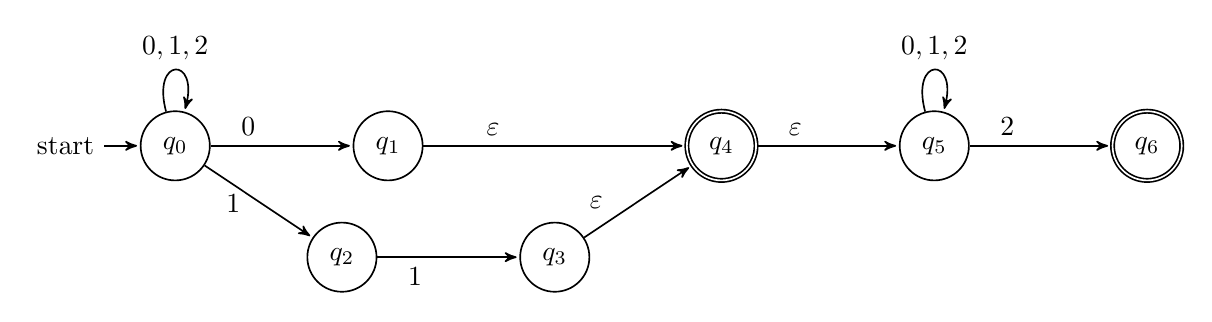
\begin{tikzpicture}[->,>=stealth',shorten >=1pt, auto, node distance=2cm, semithick]
   \tikzstyle{every state}=[text=black, fill=none]
   
   \node[initial,state] (q0)          {$q_0$};
   \node[state]         (q1) [right of=q0, xshift=20pt] {$q_1$};
   \node[state]         (q2) [below right of=q0, xshift=20pt] {$q_2$};
   \node[state]         (q3) [right of=q2, xshift=20pt] {$q_3$};
   \node[state, accepting]         (q4) [above right of=q3, xshift=20pt] {$q_4$};
   \node[state]         (q5) [right of=q4, xshift=20pt] {$q_5$};
   \node[state, accepting]         (q6) [right of=q5, xshift=20pt] {$q_6$};
   
   \path (q0) edge  [loop above] node {$0,1,2$} (q0)
           edge [bend right=0, near start] node[above] {$0$} (q1)
           edge [bend left=0, near start] node[below] {$1$} (q2)
       (q1) edge [bend left=0, near start] node {$\varepsilon$} (q4)
       (q2) edge [bend left=0, near start] node[below] {$1$} (q3)
       (q3) edge [bend left=0, near start] node {$\varepsilon$} (q4)
       (q4) edge [bend left=0, near start] node {$\varepsilon$} (q5)
       (q5) edge [loop above] node {$0,1,2$} (q5)
       (q5) edge [bend left=0, near start] node {$2$} (q6)
   ;
   \end{tikzpicture}

    \begin{enumerate}
      \item\gradeCompleteFirst Give two examples of strings of length greater than $2$ 
      that are accepted by $N$ and two examples of strings of length greater than $2$ 
      that are rejected by $N$. For each example string, list at least one of the 
      computations of $N$ on this string and 
      label whether this computation witnesses that the string is accepted by $N$.

      \item\gradeCorrectFirst Use the ``macro-state'' construction from Theorem 1.39 and class to create the DFA
      $M$ recognizing the same language as $N$. You only need to include states that are reachable from the start
      state. For full credit, submit (1) a state diagram that is deterministic (there should be arrows labelled $0$, $1$, and 
      $2$ coming out of each state) and where each state is labelled by a subset of the states in $N$; 
      and (2) for one of your example strings that is accepted by $N$, give the computation of $M$ on this string as a 
      seqeuence of states visited; and (3) for one of your example strings that is rejected by $N$, 
      give the computation of $M$ on this string as a seqeuence of states visited.

      \item\gradeComplete Give a mathematical description either using set builder notation or a regular expression
      for $L(N)$ and for $L(M)$.
    \end{enumerate}

%%%%%%%%%%% PROBLEM 2 %%%%%%%%%%%
\item \textbf{Multiple representations} (12 points):

\begin{enumerate}
   \item Consider the language $A_1 = \{ uw \mid \text{$u$ and
   $w$ are strings over $\{0,1\}$ and have the same length} \}$
   and the following argument.

   \begin{quote}
      ``Proof" that $A_1$ is not regular using the Pumping Lemma: Let $p$ be 
      an arbitrary positive integer. We will show that $p$ is not a pumping length for $A_1$. 
      
      Choose $s$ to be the string $1^p 0^p$, which is in $A_1$ because
      we can choose $u = 1^p$ and $w = 0^p$ which each have length $p$.
      Since $s$ is in $A_1$ and has length greater than or equal to $p$, if $p$ were to be a
      pumping length for $A_1$, $s$ ought to be pump'able. 
      That is, there should be a way of dividing $s$ into parts $x,y,z$ where $s=xyz$,
      $|y| >0$, $|xy| \leq p$, and for each $i \geq 0$, $xy^iz \in A_1$.
      Suppose $x,y,z$ are such that $s = xyz$, $|y| > 0$ and $|xy| \leq p$.
      Since the first $p$ letters of $s$ are all $1$ and $|xy| \leq p$, we know
      that $x$ and $y$ are made up of all $1$s.  If we let $i=2$, we get 
      a string $xy^iz$ that is not in $A_1$ because repeating $y$ twice adds $1$s to 
      $u$ but not to $w$, and strings in $A_1$ are required to have $u$ and $w$ be the same
      length. Thus, $s$ is not pumpable (even though it should have been if $p$ were to be a pumping length)
      and so $p$ is not a pumping length for $A_1$.  Since $p$ was arbitrary, we have
      demonstrated that $A_1$ has no pumping length.  By the Pumping Lemma, this implies that 
      $A_1$ is nonregular.
      \end{quote}
      \begin{enumerate}
         \item \gradeComplete Find the (first and/or most significant) logical error in the ``proof" above 
         and describe why it's wrong.
   
         \item \gradeComplete Prove that the set $A_1$ is actually regular (by finding a regular expression that describes it or 
         a DFA/NFA that recognizes it, and justifying why) {\bf or} fix the proof so that it is logically sound.     
      \end{enumerate}

   \item Consider the language $A_2 = \{ u1w \mid \text{$u$ and
   $w$ are strings over $\{0,1\}$ and have the same length} \}$
   and the following argument.


   \begin{quote}
      ``Proof" that $A_2$ is not regular using the Pumping Lemma: Let $p$ be 
      an arbitrary positive integer. We will show that $p$ is not a pumping length for $A_2$. 
      
      Choose $s$ to be the string $1^{p+1} 0^{p}$, which is in $A_2$ because
      we can choose $u = 1^p$ and $w = 0^p$ which each have length $p$.
      Since $s$ is in $A_2$ and has length greater than or equal to $p$, if $p$ were to be a
      pumping length for $A_2$, $s$ ought to be pump'able. 
      That is, there should be a way of dividing $s$ into parts $x,y,z$ where $s=xyz$,
      $|y| >0$, $|xy| \leq p$, and for each $i \geq 0$, $xy^iz \in A_2$.
      When $x = \varepsilon$ and $y = 1^{p+1}$ and $z = 0^{p}$,
      we have satisfied that $s = xyz$, $|y| > 0$ (because $p$ is positive) and $|xy| \leq p$.
      If we let $i=0$, we get 
      the string $xy^iz = 0^{p}$ that is not in $A_2$ because its middle symbol is a $0$, not a $1$. 
      Thus, $s$ is not pumpable (even though it should have been if $p$ were to be a pumping length)
      and so $p$ is not a pumping length for $A_2$.  Since $p$ was arbitrary, we have
      demonstrated that $A_2$ has no pumping length.  By the Pumping Lemma, this implies that 
      $A_2$ is nonregular.
      \end{quote}

      \begin{enumerate}

      \item \gradeComplete Find the (first and/or most significant) logical error in the ``proof" above 
      and describe why it's wrong.

      \item \gradeComplete Prove that the set $A_2$ is actually regular (by finding a regular expression that describes it or 
      a DFA/NFA that recognizes it, and justifying why) {\bf or} fix the proof so that it is logically sound.
      
      \end{enumerate}
   
\end{enumerate}


%%%%%%%%%%% PROBLEM 3 %%%%%%%%%%%
\item \textbf{Pumping} (10 points):

\begin{enumerate}
\item\gradeCorrect Give an example of a language
over the alphabet $\{a,b\}$ that has cardinality $5$ and for which $4$ is a pumping length
and $3$ is not a pumping length. Is this language regular? A complete solution will give 
(1) a clear and precise
description of the language, (2) a justification for why $4$ is a pumping length, (3) a 
justification for why $3$ is not a pumping length, (4) a correct and justified answer to 
whether the language is regular.


\item\gradeComplete In class and in the reading so far, we've seen the following examples of nonregular sets:
\begin{multicols}{3}
\begin{center}
$\{ 0^n 1^n ~|~ n \geq 0 \}$
$$\{ 0^n 1^n ~|~ n \geq 2 \}$$
$$\{ 0^n 1^m ~|~  0 \leq n \leq m \}$$
$$\{ 0^n 1^m ~|~ 0 \leq m \leq n \}$$
$$\{ 0^i 1^{2i} ~|~ 0 \leq i \}$$
$$\{ 0^i 1^{i+1} ~|~ 0 \leq i \}$$
$$\{ 0^n 1^m 0^n ~|~n,m \geq 0\}$$
$$\{ w \in \{0,1\}^* ~|~w = w^R\}$$
$$\{ w w^R ~|~ w \in \{0,1\}^*\}$$
\end{center}
\end{multicols}
Modify one of these sets in some way and use the Pumping Lemma to prove that the resulting set is still nonregular.

\end{enumerate}

%%%%%%%%%%% PROBLEM 4 %%%%%%%%%%%
\item\textbf{Regular and nonregular languages} (12 points):
In Week 2's review quiz, we saw the definition that a set $X$ is said to be 
{\bf closed under an operation} if, for any elements in
$X$, applying to them gives an element in $X$. For example, the set of
integers is closed under multiplication because if we take any two
integers, their product is also an integer .

Prove or disprove each closure claim statement below about the class of regular languages
and the class of nonregular languages.
Your arguments may refer to theorems proved in the textbook and class, and if they do, should 
include specific page numbers and references (i.e.\ write out the claim that was proved in the book 
and/or class).

Recall the definitions we have: 

For language $L$ over the alphabet $\Sigma_1 = \{0,1\}$, we have the 
associated sets of strings
\[
   SUBSTRING(L) = \{ w \in \Sigma_1^* ~|~ \text{there exist } a,b \in \Sigma_1^* \text{ such that } awb \in L\}
\]
and 
\[
  EXTEND(L) = \{ w \in \Sigma_1^* ~|~ w = uv \text{ for some strings } u \in L \text{ and } v \in \Sigma_1^* \}
\]
\begin{enumerate} 
   \item \gradeComplete The set of regular languages over $\{0,1\}$ is closed under the $SUBSTRING$ operation.

   \item \gradeComplete The set of nonregular languages over $\{0,1\}$ is closed under the $SUBSTRING$ operation.

   \item \gradeCorrect The set of regular languages over $\{0,1\}$ is closed under the $EXTEND$ operation.

   \item \gradeCorrect The set of nonregular languages over $\{0,1\}$ is closed under the $EXTEND$ operation.
\end{enumerate}

\end{enumerate}
\end{document}